\documentclass[8pt,aspectratio=169]{beamer}
\usetheme{Madrid}
\usepackage{graphicx,booktabs,adjustbox,multicol,amsmath,amssymb,listings,xcolor}
\definecolor{mlblue}{RGB}{0,102,204}
\definecolor{mlpurple}{RGB}{51,51,178}
\definecolor{mllavender}{RGB}{173,173,224}
\definecolor{mllavender2}{RGB}{193,193,232}
\definecolor{mllavender3}{RGB}{204,204,235}
\definecolor{mllavender4}{RGB}{214,214,239}
\definecolor{mlorange}{RGB}{255,127,14}
\definecolor{mlgreen}{RGB}{44,160,44}
\definecolor{mlred}{RGB}{214,39,40}
\definecolor{mlgray}{RGB}{127,127,127}
\definecolor{solkeyword}{RGB}{0,102,153}
\setbeamercolor{palette primary}{bg=mllavender3,fg=mlpurple}
\setbeamercolor{palette secondary}{bg=mllavender2,fg=mlpurple}
\setbeamercolor{palette tertiary}{bg=mllavender,fg=white}
\setbeamercolor{palette quaternary}{bg=mlpurple,fg=white}
\setbeamercolor{structure}{fg=mlpurple}
\setbeamercolor{title}{fg=mlpurple}
\setbeamercolor{frametitle}{fg=mlpurple,bg=mllavender3}
\setbeamercolor{block title}{bg=mllavender2,fg=mlpurple}
\setbeamercolor{block body}{bg=mllavender4,fg=black}
\setbeamertemplate{navigation symbols}{}
\setbeamertemplate{itemize items}[circle]
\setbeamersize{text margin left=5mm,text margin right=5mm}
\newcommand{\bottomnote}[1]{\vfill\vspace{-2mm}\textcolor{mllavender2}{\rule{\textwidth}{0.4pt}}\vspace{1mm}\footnotesize\textbf{#1}}
\usepackage{tikz,pgfplots}
\pgfplotsset{compat=1.18}
\usetikzlibrary{arrows.meta,positioning,shapes.geometric,calc}
\title{Introduction to Smart Contracts: Course Preview}
\subtitle{INTRO Preview}
\author{Prof.~Dr.~Joerg Osterrieder}
\institute{University Lecture Series}
\date{\today}
\begin{document}

% Frame 1: Title
\begin{frame}
\titlepage
\end{frame}

% Frame 2: Why Smart Contracts Matter
\begin{frame}{Why Smart Contracts Matter}
\begin{columns}[T]
\begin{column}{0.62\textwidth}
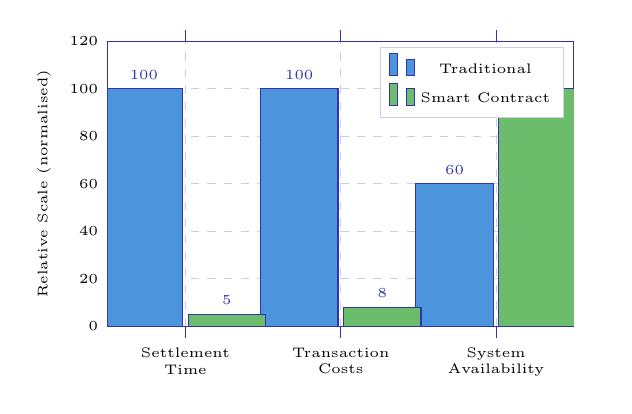
\begin{tikzpicture}
\begin{axis}[
  ybar,
  bar width=28pt,
  width=7.5cm,
  height=5.2cm,
  symbolic x coords={Settlement, Costs, Availability},
  xtick=data,
  xticklabels={Settlement\\Time, Transaction\\Costs, System\\Availability},
  xticklabel style={font=\tiny, text width=2.5cm, align=center},
  ymin=0, ymax=120,
  ytick={0,20,40,60,80,100,120},
  yticklabel style={font=\tiny},
  ylabel style={font=\tiny},
  ylabel={Relative Scale (normalised)},
  axis line style={draw=mlpurple},
  tick style={draw=mlpurple},
  nodes near coords,
  nodes near coords style={font=\tiny, color=mlpurple},
  point meta=y,
  enlarge x limits=0.25,
  grid=major,
  grid style={dashed, mllavender3},
  legend style={at={(0.98,0.98)}, anchor=north east, font=\tiny, draw=mllavender3},
]
\addplot[fill=mlblue!70, draw=mlpurple] coordinates {(Settlement,100) (Costs,100) (Availability,60)};
\addplot[fill=mlgreen!70, draw=mlpurple] coordinates {(Settlement,5) (Costs,8) (Availability,100)};
\legend{Traditional, Smart Contract}
\end{axis}
\end{tikzpicture}
\end{column}
\begin{column}{0.36\textwidth}
\vspace{4mm}
\begin{block}{Key Advantages}
\begin{itemize}\setlength\itemsep{4pt}
  \item[\small$\checkmark$] \small \textbf{95\% faster} settlement (seconds vs days)
  \item[\small$\checkmark$] \small \textbf{90\% lower} transaction costs
  \item[\small$\checkmark$] \small \textbf{24/7/365} availability, no downtime
  \item[\small$\checkmark$] \small \textbf{100\% transparent} and auditable
\end{itemize}
\end{block}
\end{column}
\end{columns}
\bottomnote{Smart contracts dramatically reduce settlement times and costs while providing round-the-clock availability that traditional systems cannot match.}
\end{frame}

% Frame 3: From Paper Contracts to Code
\begin{frame}{From Paper Contracts to Code}
\vspace{2mm}
\begin{center}
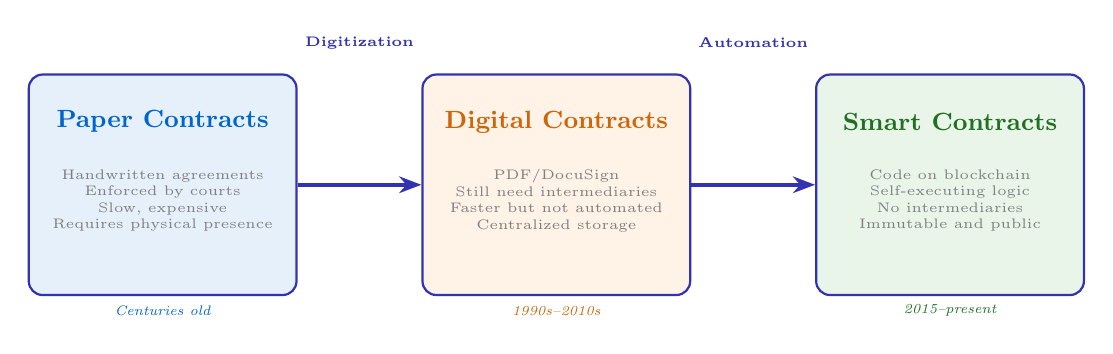
\begin{tikzpicture}[
  evo/.style={rectangle, rounded corners=5pt, draw=mlpurple, thick,
              minimum width=3.4cm, minimum height=2.8cm, align=center, fill=#1},
  elbl/.style={font=\small\bfseries, text=#1},
  edesc/.style={font=\tiny, text=mlgray, align=center, text width=3.0cm},
  arr/.style={-{Stealth[length=8pt]}, ultra thick, draw=mlpurple}
]
% Stage 1: Paper
\node[evo=mlblue!10] (paper) at (0,0) {};
\node[elbl=mlblue] at (0,0.8) {Paper Contracts};
\node[edesc] at (0,-0.2) {Handwritten agreements\\Enforced by courts\\Slow, expensive\\Requires physical presence};
\node[font=\tiny\itshape, text=mlblue] at (0,-1.6) {Centuries old};

% Stage 2: Digital
\node[evo=mlorange!10] (digital) at (5,0) {};
\node[elbl=mlorange!80!black] at (5,0.8) {Digital Contracts};
\node[edesc] at (5,-0.2) {PDF/DocuSign\\Still need intermediaries\\Faster but not automated\\Centralized storage};
\node[font=\tiny\itshape, text=mlorange!80!black] at (5,-1.6) {1990s--2010s};

% Stage 3: Smart Contract
\node[evo=mlgreen!10] (smart) at (10,0) {};
\node[elbl=mlgreen!70!black] at (10,0.8) {Smart Contracts};
\node[edesc] at (10,-0.2) {Code on blockchain\\Self-executing logic\\No intermediaries\\Immutable and public};
\node[font=\tiny\itshape, text=mlgreen!70!black] at (10,-1.6) {2015--present};

% Arrows
\draw[arr] (paper.east) -- (digital.west);
\draw[arr] (digital.east) -- (smart.west);

% Progress labels
\node[font=\tiny, text=mlpurple] at (2.5,1.8) {\textbf{Digitization}};
\node[font=\tiny, text=mlpurple] at (7.5,1.8) {\textbf{Automation}};
\end{tikzpicture}
\end{center}
\bottomnote{The evolution from paper to smart contracts represents a shift from human-enforced agreements to machine-enforced, trustless execution on a global ledger.}
\end{frame}

% Frame 4: The Smart Contract Stack
\begin{frame}{The Smart Contract Stack}
\vspace{2mm}
\begin{center}
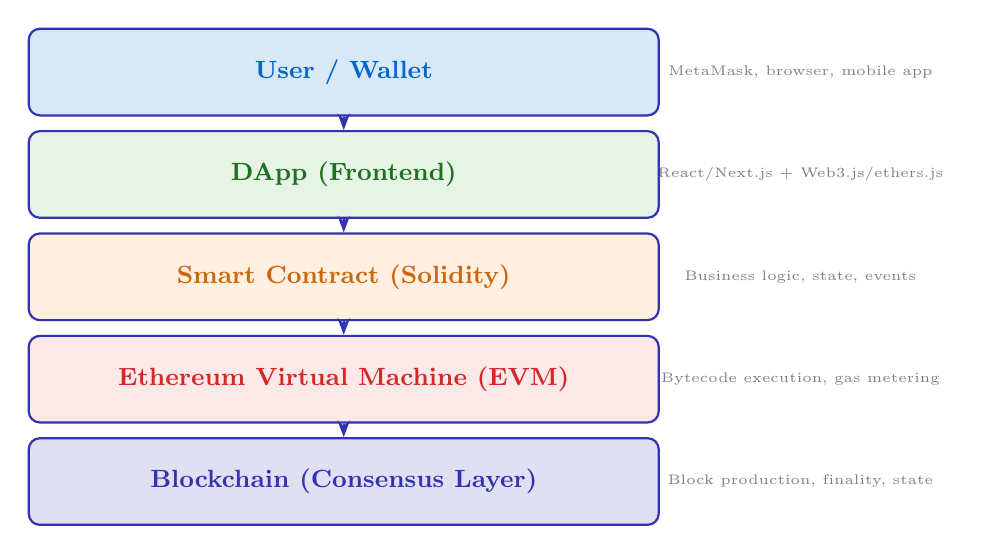
\begin{tikzpicture}[
  layer/.style={rectangle, rounded corners=4pt, draw=mlpurple, thick,
                minimum width=8cm, minimum height=1.1cm,
                font=\small\bfseries, align=center},
  ldesc/.style={font=\tiny, text=mlgray, align=left},
  arr/.style={-{Stealth[length=6pt]}, thick, draw=mlpurple}
]
% Layer 5 (top): User
\node[layer, fill=mlblue!15, text=mlblue] (user) at (0,4.0) {User / Wallet};
\node[ldesc] at (5.8,4.0) {MetaMask, browser, mobile app};

% Layer 4: DApp
\node[layer, fill=mlgreen!12, text=mlgreen!70!black] (dapp) at (0,2.7) {DApp (Frontend)};
\node[ldesc] at (5.8,2.7) {React/Next.js + Web3.js/ethers.js};

% Layer 3: Smart Contract
\node[layer, fill=mlorange!12, text=mlorange!80!black] (contract) at (0,1.4) {Smart Contract (Solidity)};
\node[ldesc] at (5.8,1.4) {Business logic, state, events};

% Layer 2: EVM
\node[layer, fill=mlred!10, text=mlred] (evm) at (0,0.1) {Ethereum Virtual Machine (EVM)};
\node[ldesc] at (5.8,0.1) {Bytecode execution, gas metering};

% Layer 1 (bottom): Blockchain
\node[layer, fill=mlpurple!15, text=mlpurple] (chain) at (0,-1.2) {Blockchain (Consensus Layer)};
\node[ldesc] at (5.8,-1.2) {Block production, finality, state};

% Arrows
\draw[arr] (user.south) -- (dapp.north);
\draw[arr] (dapp.south) -- (contract.north);
\draw[arr] (contract.south) -- (evm.north);
\draw[arr] (evm.south) -- (chain.north);
\end{tikzpicture}
\end{center}
\bottomnote{Users interact through wallets and DApps; transactions flow down through smart contracts and the EVM to the consensus layer for permanent recording.}
\end{frame}

% Frame 5: What You Will Learn
\begin{frame}{What You Will Learn}
\begin{columns}[T]
\begin{column}{0.44\textwidth}
\vspace{2mm}
\begin{block}{Learning Outcomes}
\begin{itemize}\setlength\itemsep{5pt}
  \item[\small$\checkmark$] \small \textbf{Foundations} --- history from Szabo to Ethereum, contract lifecycle and deployment
  \item[\small$\checkmark$] \small \textbf{Solidity \& EVM} --- data types, functions, storage vs memory, gas optimization
  \item[\small$\checkmark$] \small \textbf{Design patterns} --- proxy, factory, access control, upgradeability
  \item[\small$\checkmark$] \small \textbf{Security} --- reentrancy, integer overflow, oracle manipulation, auditing
  \item[\small$\checkmark$] \small \textbf{Applications} --- DeFi protocols, NFT marketplaces, DAOs, supply chain
\end{itemize}
\end{block}
\end{column}
\begin{column}{0.54\textwidth}
\vspace{2mm}
\begin{center}
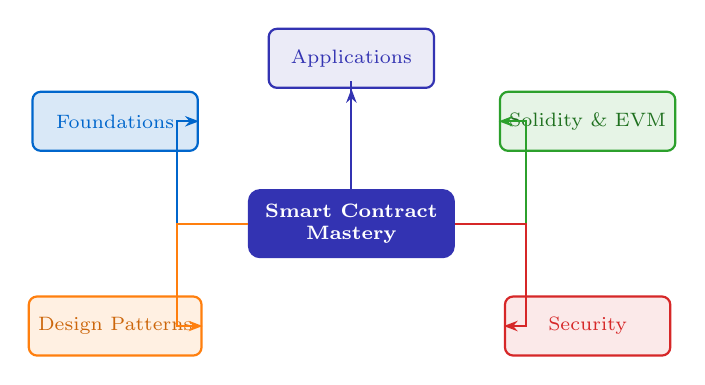
\begin{tikzpicture}[
  cbox/.style={rectangle, rounded corners=4pt, draw=mlpurple, thick,
               fill=mlpurple, minimum width=2.6cm, minimum height=0.85cm,
               font=\scriptsize\bfseries, align=center, text=white},
  fbox/.style={rectangle, rounded corners=3pt, thick,
               minimum width=2.1cm, minimum height=0.75cm,
               font=\scriptsize, align=center},
  farr/.style={-{Stealth[length=5pt]}, thick}
]
% Central node
\node[cbox] (nm) at (0,0) {Smart Contract\\Mastery};

% Skill nodes
\node[fbox, draw=mlblue,   fill=mlblue!15,   text=mlblue]              (found) at (-3.0, 1.3) {Foundations};
\node[fbox, draw=mlgreen,  fill=mlgreen!12,  text=mlgreen!70!black]    (sol)   at ( 3.0, 1.3) {Solidity \& EVM};
\node[fbox, draw=mlorange, fill=mlorange!12, text=mlorange!80!black]   (patt)  at (-3.0,-1.3) {Design Patterns};
\node[fbox, draw=mlred,    fill=mlred!10,    text=mlred]               (sec)   at ( 3.0,-1.3) {Security};
\node[fbox, draw=mlpurple, fill=mlpurple!10, text=mlpurple]            (apps)  at ( 0.0, 2.1) {Applications};

% Arrows
\draw[farr, draw=mlblue]   (nm.west)  -- ++(-0.9,0) |- (found.east);
\draw[farr, draw=mlgreen]  (nm.east)  -- ++(0.9,0)  |- (sol.west);
\draw[farr, draw=mlorange] (nm.west)  -- ++(-0.9,0) |- (patt.east);
\draw[farr, draw=mlred]    (nm.east)  -- ++(0.9,0)  |- (sec.west);
\draw[farr, draw=mlpurple] (nm.north) -- ++(0,0.6)  |- (apps.south);
\end{tikzpicture}
\end{center}
\end{column}
\end{columns}
\vspace{1mm}
\bottomnote{By the end you will be able to read, write, audit, and deploy smart contracts with awareness of security trade-offs and real-world applications.}
\end{frame}

% Frame 6: Course Roadmap
\begin{frame}{Course Roadmap}
\vspace{2mm}
\begin{center}
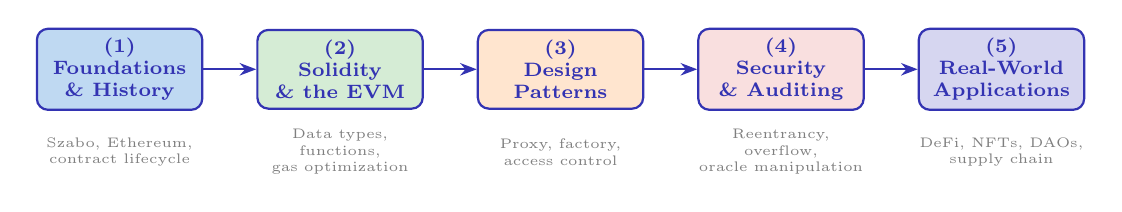
\begin{tikzpicture}[
  milestone/.style={rectangle, rounded corners=4pt, draw=mlpurple, thick,
                    minimum width=2.1cm, minimum height=1.0cm,
                    fill=mllavender3, font=\scriptsize\bfseries,
                    align=center, text=mlpurple},
  conn/.style={-{Stealth[length=6pt]}, thick, draw=mlpurple}
]
\node[milestone, fill=mlblue!25]    (m1) at (0,0)    {(1)\\Foundations\\\& History};
\node[milestone, fill=mlgreen!20]   (m2) at (2.8,0)  {(2)\\Solidity\\\& the EVM};
\node[milestone, fill=mlorange!20]  (m3) at (5.6,0)  {(3)\\Design\\Patterns};
\node[milestone, fill=mlred!15]     (m4) at (8.4,0)  {(4)\\Security\\\& Auditing};
\node[milestone, fill=mlpurple!20]  (m5) at (11.2,0) {(5)\\Real-World\\Applications};

\draw[conn] (m1) -- (m2);
\draw[conn] (m2) -- (m3);
\draw[conn] (m3) -- (m4);
\draw[conn] (m4) -- (m5);

\node[font=\tiny, text=mlgray, align=center, text width=2.1cm] at (0,-1.05)
  {Szabo, Ethereum,\\contract lifecycle};
\node[font=\tiny, text=mlgray, align=center, text width=2.1cm] at (2.8,-1.05)
  {Data types, functions,\\gas optimization};
\node[font=\tiny, text=mlgray, align=center, text width=2.1cm] at (5.6,-1.05)
  {Proxy, factory,\\access control};
\node[font=\tiny, text=mlgray, align=center, text width=2.1cm] at (8.4,-1.05)
  {Reentrancy, overflow,\\oracle manipulation};
\node[font=\tiny, text=mlgray, align=center, text width=2.1cm] at (11.2,-1.05)
  {DeFi, NFTs, DAOs,\\supply chain};
\end{tikzpicture}
\end{center}
\vspace{4mm}
\begin{columns}[T]
\begin{column}{0.48\textwidth}
\begin{block}{Prerequisites}
\begin{itemize}\setlength\itemsep{2pt}
  \item[\small$\checkmark$] \small Basic blockchain and cryptography concepts
  \item[\small$\checkmark$] \small Familiarity with any programming language
\end{itemize}
\end{block}
\end{column}
\begin{column}{0.48\textwidth}
\begin{block}{Outcomes}
\begin{itemize}\setlength\itemsep{2pt}
  \item[\small$\checkmark$] \small Read, write, and audit Solidity smart contracts
  \item[\small$\checkmark$] \small Deploy contracts and build DApp front-ends
\end{itemize}
\end{block}
\end{column}
\end{columns}
\bottomnote{From historical origins to production deployment in five interconnected modules covering language, patterns, security, and applications.}
\end{frame}

\end{document}
